\chapter{\label{chapter3} The Abstract Syntax Tree (AST)}

The abstract class \texttt{ASTNode.cs} represents the building block of the data structure that is used as the Intermediate Representation (IR) for the \fwap language. The Abstract Syntax Tree (AST), assembled using the methods provided by the \texttt{ASTGenerator.cs} class, is the input for either the interpreter (see Chapter~\ref{chapter4}) and the \fsharp code generator (see Chapter~\ref{chapter5}). As said before, it is up to the parser, opportunely guided by the semantics annotations of Coco/R, to create the AST related to a certain \fwap source file.

\section{\texttt{Node}'s and \texttt{Term}'s}

The subclasses of \texttt{ASTNode.cs} act as a single node of the AST of a program and can be:
\begin{itemize}
	\item a \texttt{Node}, meaning an internal node of the tree 
	\item a \texttt{Term}, meaning a leaf of the tree.
\end{itemize}

Each and every \texttt{Node} is distinguished by a label which describes its function and has possibly got a list of children nodes (\texttt{List<ASTNode> children}). All the allowed labels are listed below.\\

\begin{stlisting}[caption=Labels for \texttt{Node}s.]
public enum Labels {Program, Main, Afun, FunDecl, For,
If, While, Block, Assig, Decl, AssigDecl, Return, 
Async, Print, Read, Dsync, Plus, Mul, Minus, Div, Gt,
Gte, Lt, Lte, Eq, NotEq, And, Or, Negativ, Bracket, 
FunCall};
\end{lstlisting}

\texttt{Term}'s contain a generic \texttt{object} that could be one among an integer, a boolean, a string or an \texttt{Obj} that acts as a variable (see Section\ref{typecheck}).

\section{Building the AST}

The following pictures illustrate how some labeled \texttt{Node}'s are built by the parser. An agreement on the order of the children from left to right was inevitable for implementing the interpreter and the \fsharp compiler.

\newpage
\begin{figure}
	\centering
		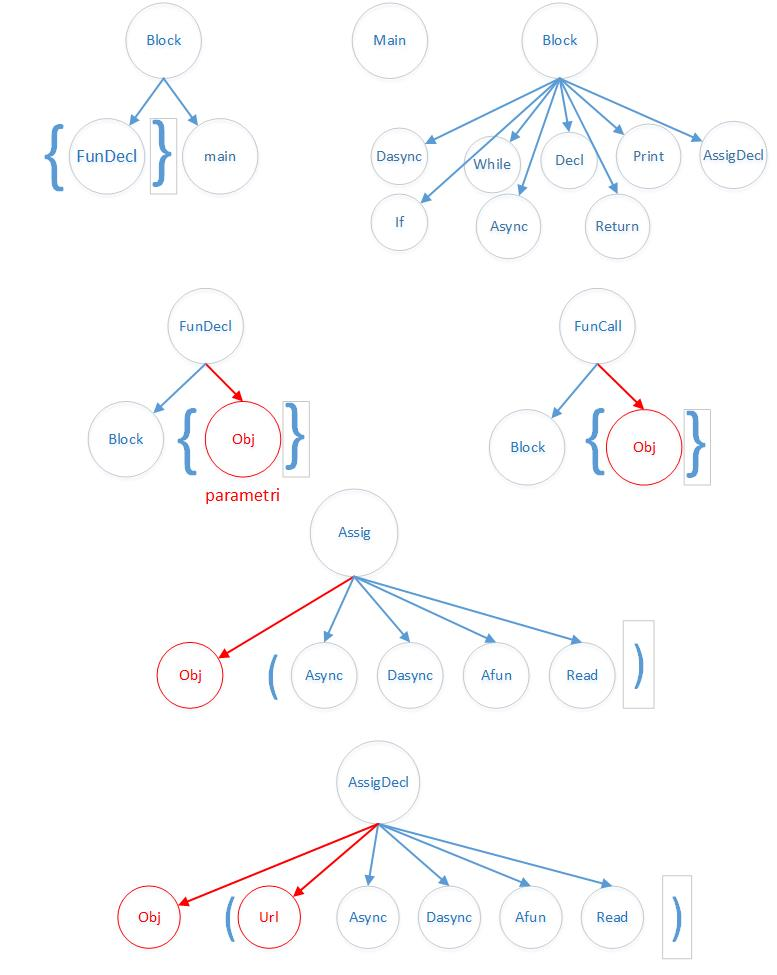
\includegraphics[width=0.90\textwidth]{C:/Users/Stefano/Documents/GitHub/APproject/docs/nodesAST/Program.jpg}
	\caption{Order of the children of some labeled \texttt{Node}'s; curly braces indicates zero or n copies of a certain node, round braces a choice among a few options.}
	\label{fig:Program}
\end{figure}


